\documentclass{article}
\usepackage{graphicx} 
\usepackage{amsfonts} 
\usepackage{amsmath}
\usepackage{multirow}
\usepackage{tikz}
\usepackage{polski}
\usepackage{mathtools}
\usepackage{hyperref}
\usepackage{breqn}

\title{ Wskaźnik planarności w grafach Barabasi Albert }

\author{}

\date{}

\begin{document}

\maketitle

\section{Cel}
Chcemy oceniać szansę na wystąpienie podpodziału $K_{3,3}$ lub $K_5$ w grafie $G^m_n$.
Zaczynamy od pustego grafu. W każdym kroku dodajemy nową krawędź/ nowy wierzchołek z krawędzią.
Co każde dodanie krawędzi na podstawie indeksu planaraności decydujemy jaki kolor jej nadać. Każdy kolor odpowiada jednej z warstw na które rozkładamy graf.
Indeks ten liczymy dla każdej warstwy osobno.

\section{Założenia}
\begin{enumerate}
    \item Dowolne ścieżki pomiędzy wierzchołkami nie powinny wpływać na wskaźnik, ponieważ mogą zostać zkontrakowane.
    \item Wskaźnik powinien uwzględniać to, że każda krawędź może zostać użyta tylko raz.
    \item Trzeba uwzględnić to aby wierzchołki tworzyły klikę czy graf pełny dwudzielny.
\end{enumerate}

\section{Realizacja}
Weźmy pewną ścieżką $P$ w grafie: $p_1, \ldots, p_k$ i zdefiniujmy funkcję:
\begin{dmath}
    \tau(P) = \phi(p_1) \cdot (\prod_{i=2}^{k-1} \psi(p_i)) \cdot \phi(p_k)
\end{dmath}
gdzie: $\phi(p) = \frac{MIN\{d, \\\ deg(p)\}}{d}$ oraz $\psi(p) = \frac{1}{deg(p) - 1}$.
\newline
Tak zdefiniowana funkcja $\tau(P)$ zwraca wartości z przedziału $(0, 1]$. Wartość 1 oznacza, że ścieżka $P$ może zostać zkontraktowana do krawędzi łączącej dwa wierzchołki stopnia $d$ oraz wierzchołki w niej występujące nie wystąpią w innym podgrafie.
\newline
Sumując wartości $\tau(P)$ dla wszystkich ścieżek pomiędzy dwoma wierzchołkami $p_i$, $p_j$ otrzymamy 'oczekiwaną liczbę ścieżek', które mogą zostać skontraktowane do krawędzi łączącej dwa wierzchołkami stopnia o 'oczekwianym stopniu $d$' - oznaczenie $\tau(P(p_i, p_j))$.
\newline
Aby określić wartość $\tau$ dla całego grafu mnożymy $\tau$ dla ścieżek pomiędzy wierzchołkami tworzącymi potencjalne kliki oraz potencjalne pełne grafy dwudzielne.

\section{Usprawnienia obliczeniowe}
Z analizy grafów planarnych wynika, że podgrafy będące podpodziałami grafów $K_{3,3}$ oraz $K_5$ mają rozmiar $O(log_2(n))$, zatem wystarczy w analizie wziąść pod uwagę ścieżki takiej długości.
\newline
Przy pojawianiu się nowego wierzchołka/krawędzi wystarczy zaktualizować część wartości. Można to będzie osiągnąć poprzez trzymanie jakiś dodatkowych informacji lub lekką modyfikację funkcji $\tau$.
Można do iloczynów wartości krawędzi grafów $K_{3,3}$ oraz $K_5$ zastować jakiś próg, aby wartości poniżej $0.1$ nie były brane pod uwagę. Można także liczyć logarytm wartości $\tau$ dla ścieżek aby zamienić iloczyny na sumy.

\section{Zalety}
Mając policzone wartości $\tau$ dla danych ścieżek można analizować które miejsca w grafie są problematyczne oraz szacować ile krawędzi będzie zakłócać planarność grafu.

\section{Przykład użycia}
Efekty kolorowania przy użyciu wskaźnika opisanego wyżej. Generowany jest graf BA dla parametru $m=5$ oraz $n=30$ i liczbie kolorów 3. 
Po dodaniu każdej krawędzi wyznaczany jest wskaźnik planarności dla każdej warstwy(koloru). Wierzchołki kolorowane są na podstawie najniższej wartości wskaźnika planarności.
Pod uwagę brane są wszytskie ścieżki - bez ograniczeń na długość.

\begin{figure}[h]
    \centering
    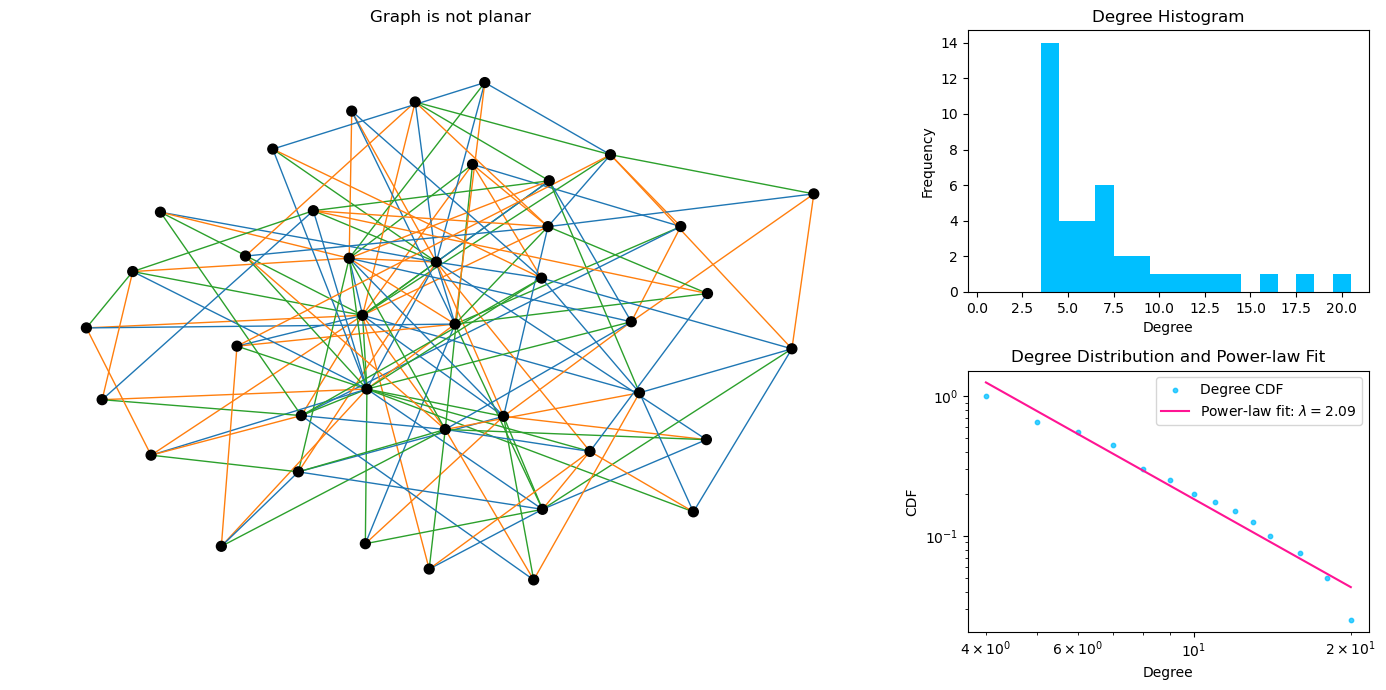
\includegraphics[width=12cm]{../images/graph.png}
\end{figure}
\begin{figure}[h]
    \centering
    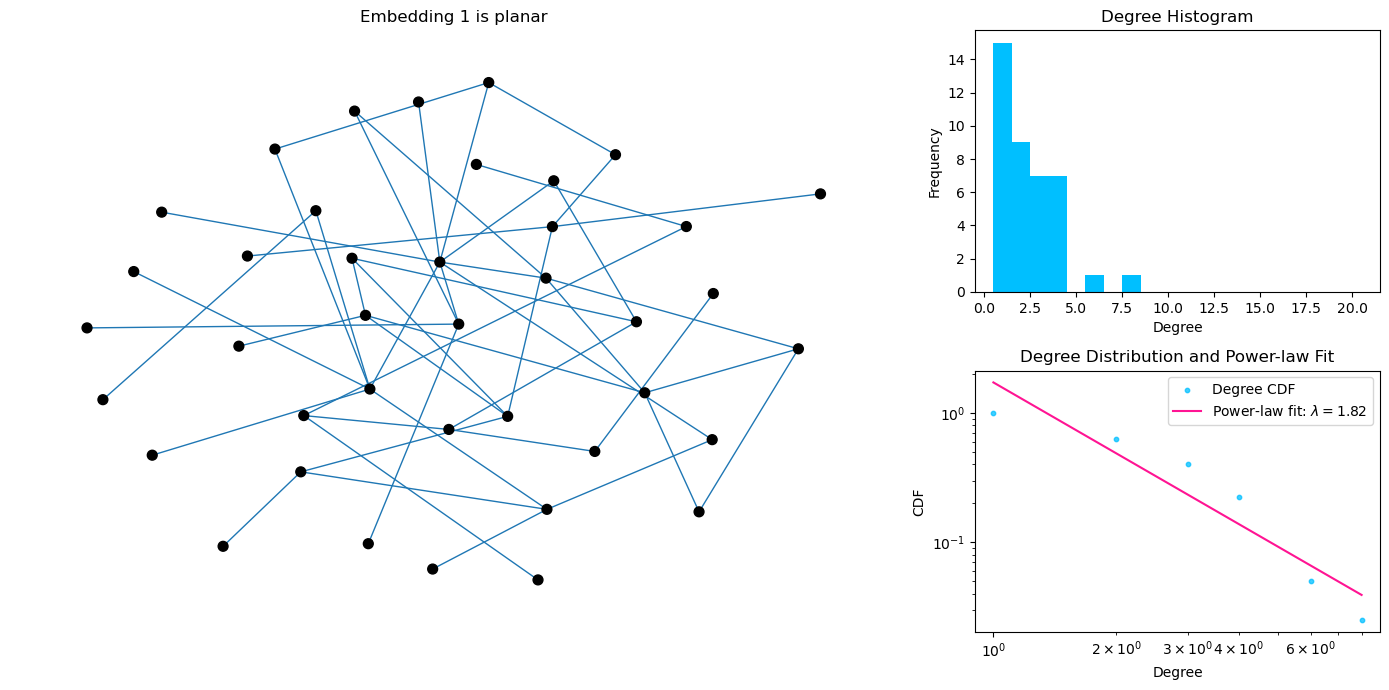
\includegraphics[width=12cm]{../images/graph-embedding1.png}
\end{figure}
\begin{figure}[h]
    \centering
    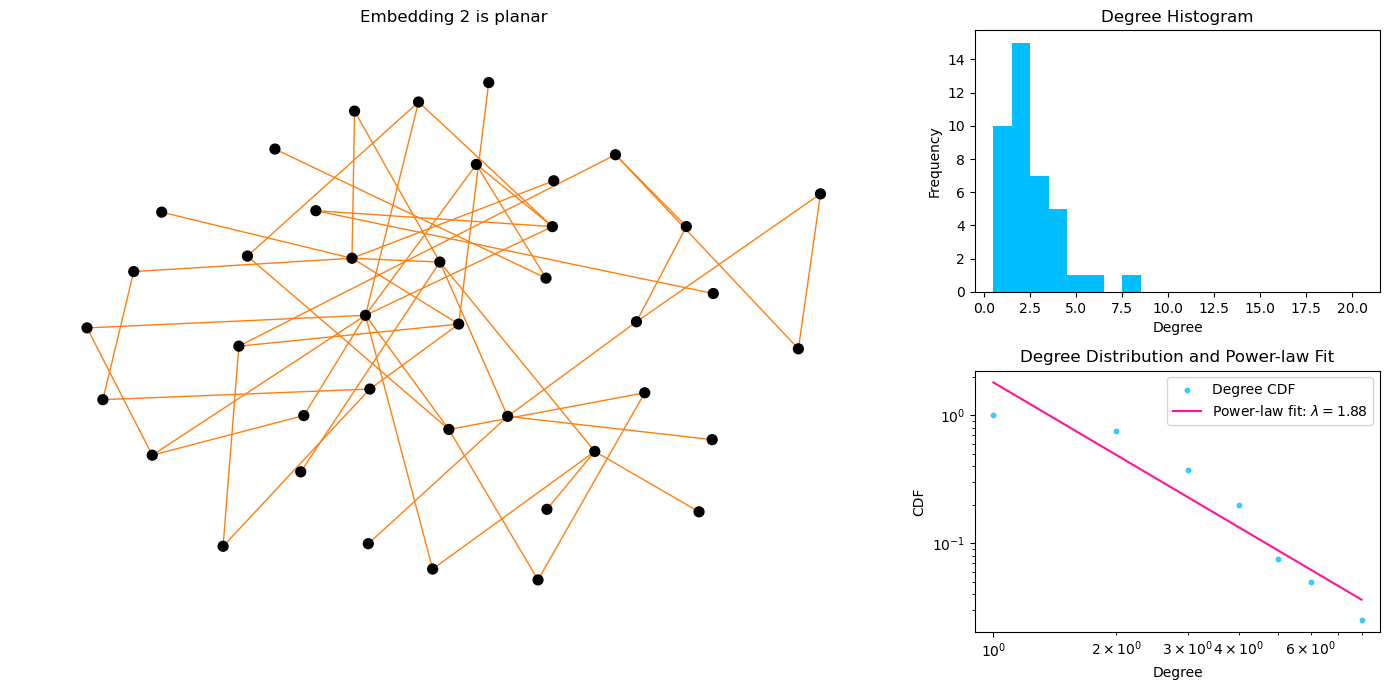
\includegraphics[width=12cm]{../images/graph-embedding2.png}
\end{figure}
\begin{figure}[h]
    \centering
    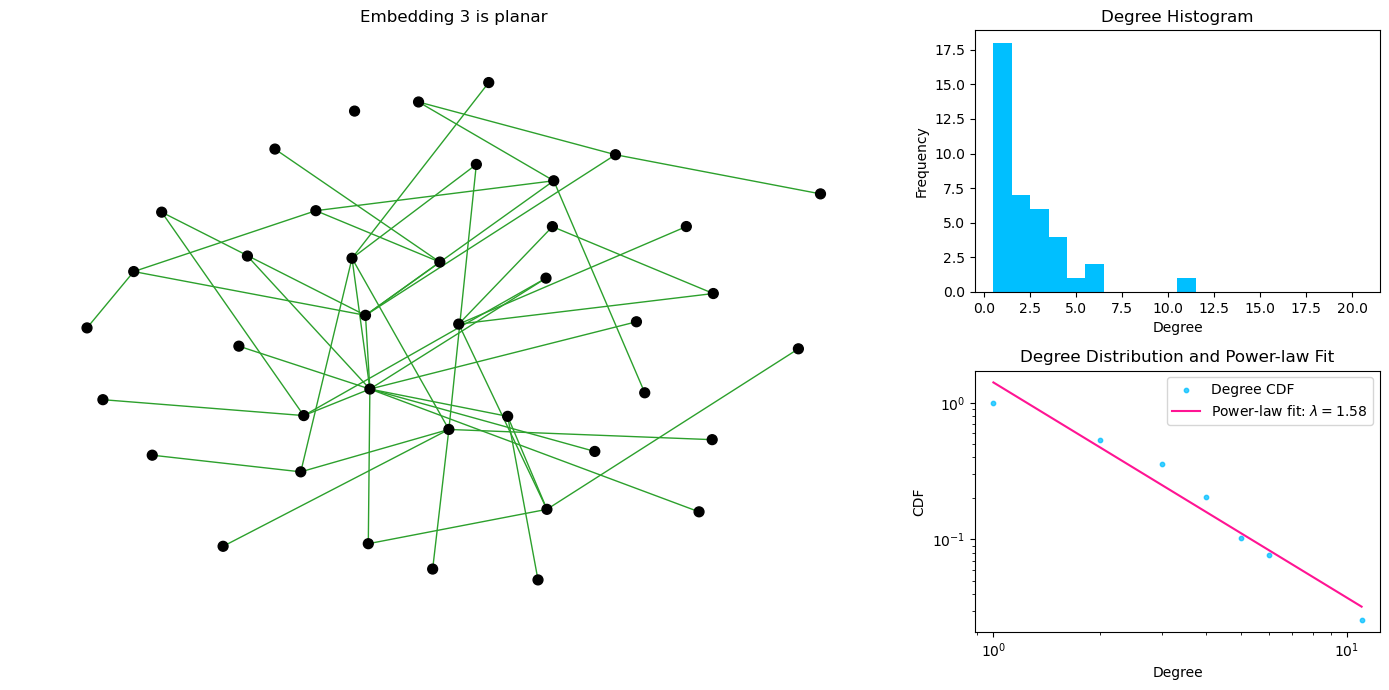
\includegraphics[width=12cm]{../images/graph-embedding3.png}
\end{figure}
\end{document}
